% Draw Hybrid Automaton Model of Thermostat in TikZ
% latexdraw.com
% 12/01/2020, 11:02

\documentclass[border=0.2cm]{standalone}

\usepackage{tikz}
\usetikzlibrary{positioning,automata}

\begin{document}

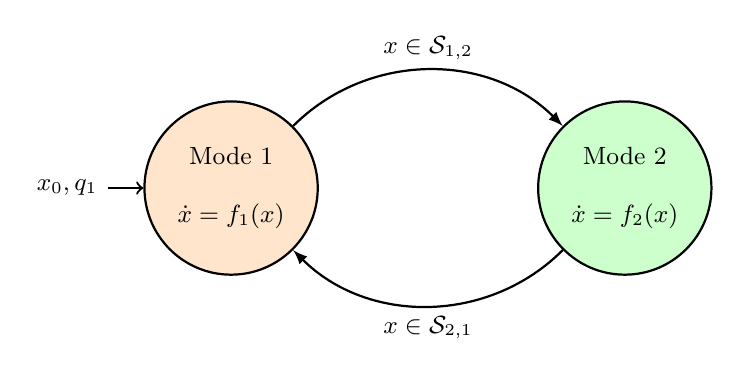
\begin{tikzpicture}[
    node distance=5cm,
    on grid,
    thick,
    font=\small]

% Mode 1    
\node[ 
    state,
    initial,
    initial text = {$x_0,q_1$},
    fill=orange!20,
    align=center,
    inner sep=5pt] (q_0) 
        {
            Mode $1$ \\[10pt]
            $\dot{x}=f_1(x)$ 
        };

% Mode 2    
\node[
    state,
    fill=green!20,
    align=center,
    inner sep=5pt] (q_1) [right=of q_0] 
        {
          Mode $2$ \\[10pt]
          $\dot{x}=f_2(x)$
        };

% Transitions
\path [-latex]
    (q_0) edge [bend left=45] 
        node [above] {
            $x\in\mathcal{S}_{1,2}$} (q_1)
    (q_1) edge [bend left=45]   
        node [below] {$x\in\mathcal{S}_{2,1}$} (q_0);
\end{tikzpicture}

\end{document} 